







\section{Measurement of the \ahe\ inelastic cross section}\label{sec:ResHe3SigmaInel}
The measurement of the \ahe\ inelastic cross section is the most fundamental result of this thesis. This is the first measurement of this inelastic cross section, which is important not just for nuclear physics, but also for astrophysical searches for physics beyond the standard model, as discussed in section \ref{sec:Intro:AntinucleiGoldenChannel}. Historically, inelastic cross section measurements were done using fixed target experiments: a beam of the particle of interest was isolated, and then fired on a material target. By measuring the abundance of the particle before and after the target, the cross section could be measured. The difficulty in doing this for antinuclei lies in the production and isolation of an antinuclei beam, since antinuclei production is so rare and has a high $\sqrt{s}$ threshold. Even at the places where antinuclei are produced (at the LHC and at high energy heavy-ion facilities\cite{}), further isolating a beam of such particles is not feasible. In fact, out of all antinuclei ($A$>2), this method has only been applied to high energy antideuterons \cite{Binon:1970yu, Denisov:1971im}, at the CERN proton synchrotron in the 70s, for particles at very high momenta of 13 GeV/$c$ and 25 GeV/$c$. Recently, roughly half a century later, the new measurement technique using the antiparticle-to-particle ratio has been shown to be able to measure the antideuteron inelastic cross section down to 500 MeV/$c$ \cite{antideuteronXS}. This measurement has now been expanded to \ahe\ \cite{antiHe3XS} and \atrit\ , and a separate complementary method (TPC/TOF method) has enabled the use of the high statistics Pb--Pb data to boost the measurements' precision. Both these new methods rely on quantifying the absorption of antinuclei as they travel through the detector material, rather than a dedicated target. The disadvantage of this approach is that the detector material is optimised to have little material budget as possible, as to not interfere with the particles of interest. Nevertheless, these methods allow us to further our knowledge of antinuclei inelastic cross sections for the first time in half a century.

\subsection{Physics motivation and overview of the analysis method}
\ahe\ nuclei are a promising probe for indirect dark matter searches, but in order to understand any potential signal, it is necessary to know their disappearance probability as they travel to earth from their cosmic sources, as is extensively discussed in sections \ref{sec:Intro:AntinucleiGoldenChannel} and \ref{sec:WIMPS}. While this is the astrophysical motivation for this measurement, it also has applications in nuclear physics. Measurements of (anti)nuclei production rely on efficiencies to be well reproduced by Monte Carlo simulation, which requires the inelastic cross sections as input. \\ 
The analysis methods are laid out below. 
\subsubsection{Antiparticle-to-particle ratio method}
\textit{The detailed steps of this method are described in section \ref{sec:ExperimentAndMethod}}\\
The antiparticle-to-particle method is based on using the ratio of antiparticles to particles as an observable for the cross section. This works since at LHC energies, matter and antimatter are produced in almost equal amounts, and therefore dividing the number of antiparticles by the number of particles acts as a normalization of the number of antiparticles produced. The detector material itself acts as a target. Since antiparticles and particles have the same interactions with the detector material apart from annihilation, uncertainties on other interactions cancel, and thus the ratio is sensitive to the inelastic cross section. 
\subsubsection{TOF-TPC matching method}\label{sec:TOFTPCMethod}
The second method for measuring \sigmainel\ uses the fact that \ahe\ can be clearly identified in the TPC, and then those tracks can be checked again in the TOF. This method works akin to a fixed target experiment, in that a "beam" is identified by measuring \ahe\ in the TPC, this beam is then fired upon the "target", which in this case is the space frame and the TRD. Some of the nuclei will annihilate, while the others who make it through will generate a matching TOF hit, thus enabling a measurement of how much of the beam survives. \\
The advantage of this method is that only the antiparticles are required; no specific assumptions about the antimatter-to-matter ratio need to be assumed and tested. This also means that secondary correction need not be applied, since the origin of the \ahe\ has no impact on the result\footnote{Also, there are no secondary \ahe\ nuclei from material spallation, so the secondary correction is even less important.}. The disadvantage is that the acceptance of the TOF detector limits the applicability of this method to higher momenta, so it is more difficult to measure the low energy rise of the inelastic cross section. \\

The measurement of \sigmainel\ using the TPC-TOF matching method is thus complementary to the antiparticle-to-particle method described above. This analysis was not carried out as part of this work, but ties in closely with the results shown both in this chapter and in chapter \ref{sec:AntinucleiInTheCosmos}, and is thus described here. The measurement is also shown together with the measurement using the antimatter-to-matter inelastic cross section. More details about the analysis can be found in \cite{PavelAN, antiHe3XS}.

\subsection{Secondary correction}
In order to extract the cross section from the antiparticle-to-particle ratio, only particles produced at the primary vertex must be considered. Thus, secondary particles need to be accounted for by using template fits, as described in section \ref{sec:Meth:secondaryCorr}. \\

The template fits done for the secondary correction of $^3\mathrm{He}$ are shown in figure \ref{fig:Template_fits_he}. The cut on |DCA$_z$| < 1 cm was chosen in order to include more secondaries, and improve the statistical constraints on the fit. As can be seen, in the first bin 

\begin{figure}
    \centering
    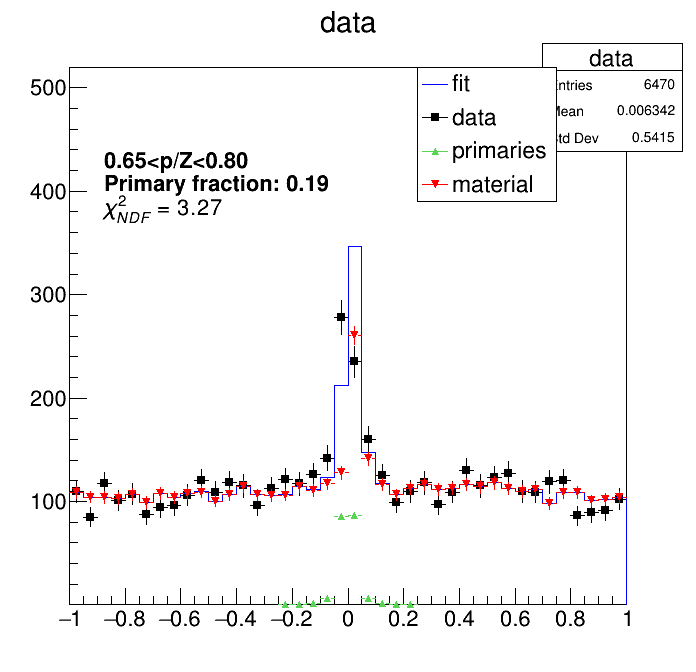
\includegraphics[width=0.32\textwidth]{figures/he3_template_fits/TemplateFitHe3_0.65<p<0.8_rebin_5.png}
    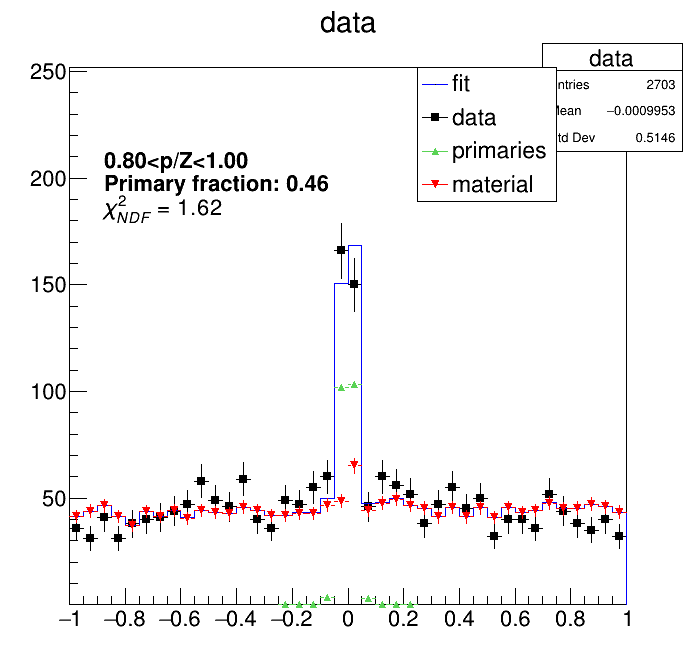
\includegraphics[width=0.32\textwidth]{figures/he3_template_fits/TemplateFitHe3_0.8<p<1.0_rebin_5.png}
    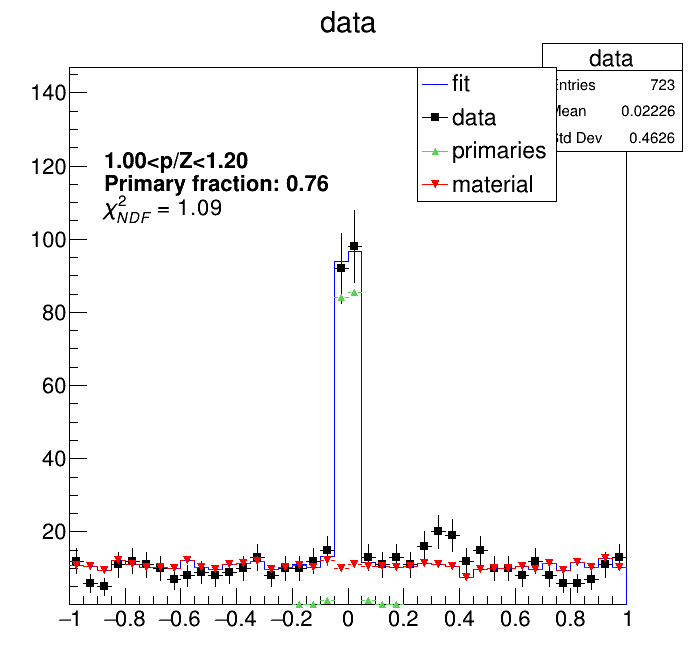
\includegraphics[width=0.32\textwidth]{figures/he3_template_fits/TemplateFitHe3_1.0<p<1.2_rebin_5.png}
    \caption{Template fits for determining the primary fraction of $^3\mathrm{He}$ in the first 3 momentum bins (above this momentum the primary fraction goes to 1), for a |DCA$_z$| < 1 cm cut. The fits were performed using the TFractionFitter method available in ROOT.}
    \label{fig:Template_fits_he}
\end{figure}

\subsection{Results}
After all the corrections are applied, we can now obtain the final \ratio\ and the corresponding \sigmainel\ , which are shown in figure \ref{fig:Ahe_sigma_inel_pp}. The measurement is in agreement with the previous parameterization used in Geant4 at a significance of slightly above 1$\sigma$. The lowest momentum bin shows a hint at a steeper rise than the parameterization. The second bin is shown as an upper limit since the uncertainties reached below 0, which would be an unphysical value for the cross section. \\

This represents the first measurement of \sigmainel\ .
\begin{figure}
    \centering
    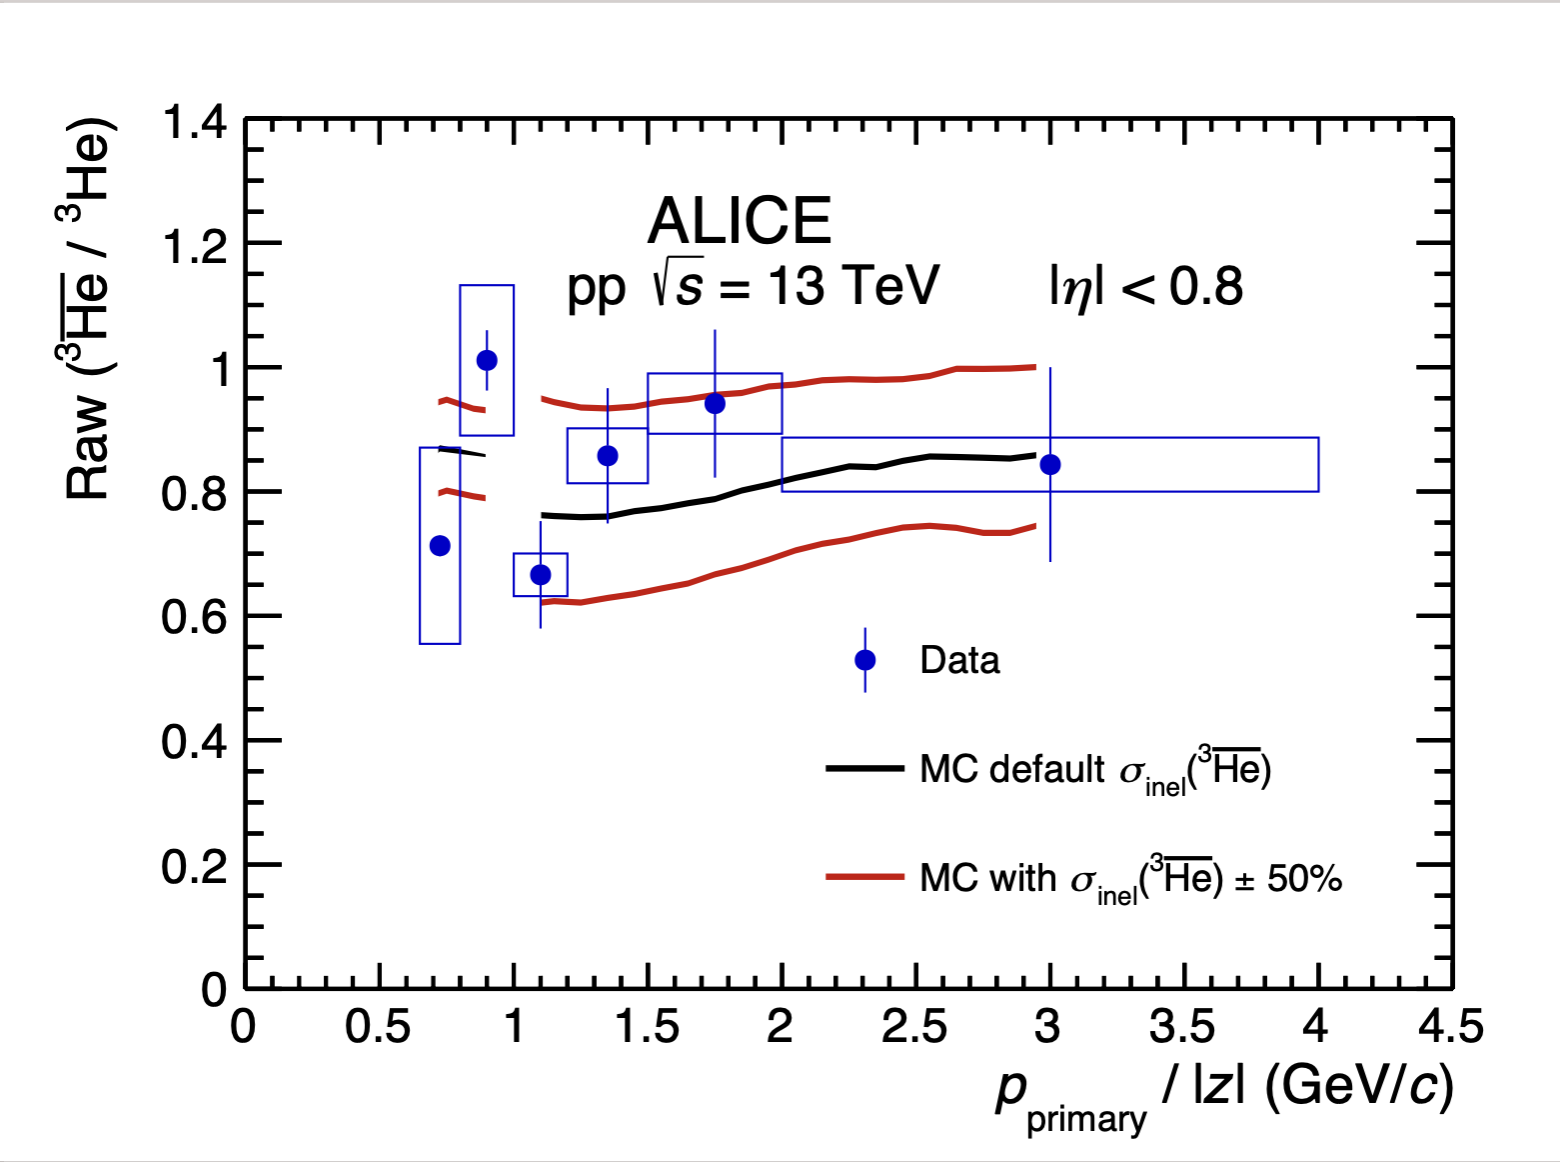
\includegraphics[width=0.48\textwidth]{figures/he3bar_he3_ratio.png}
    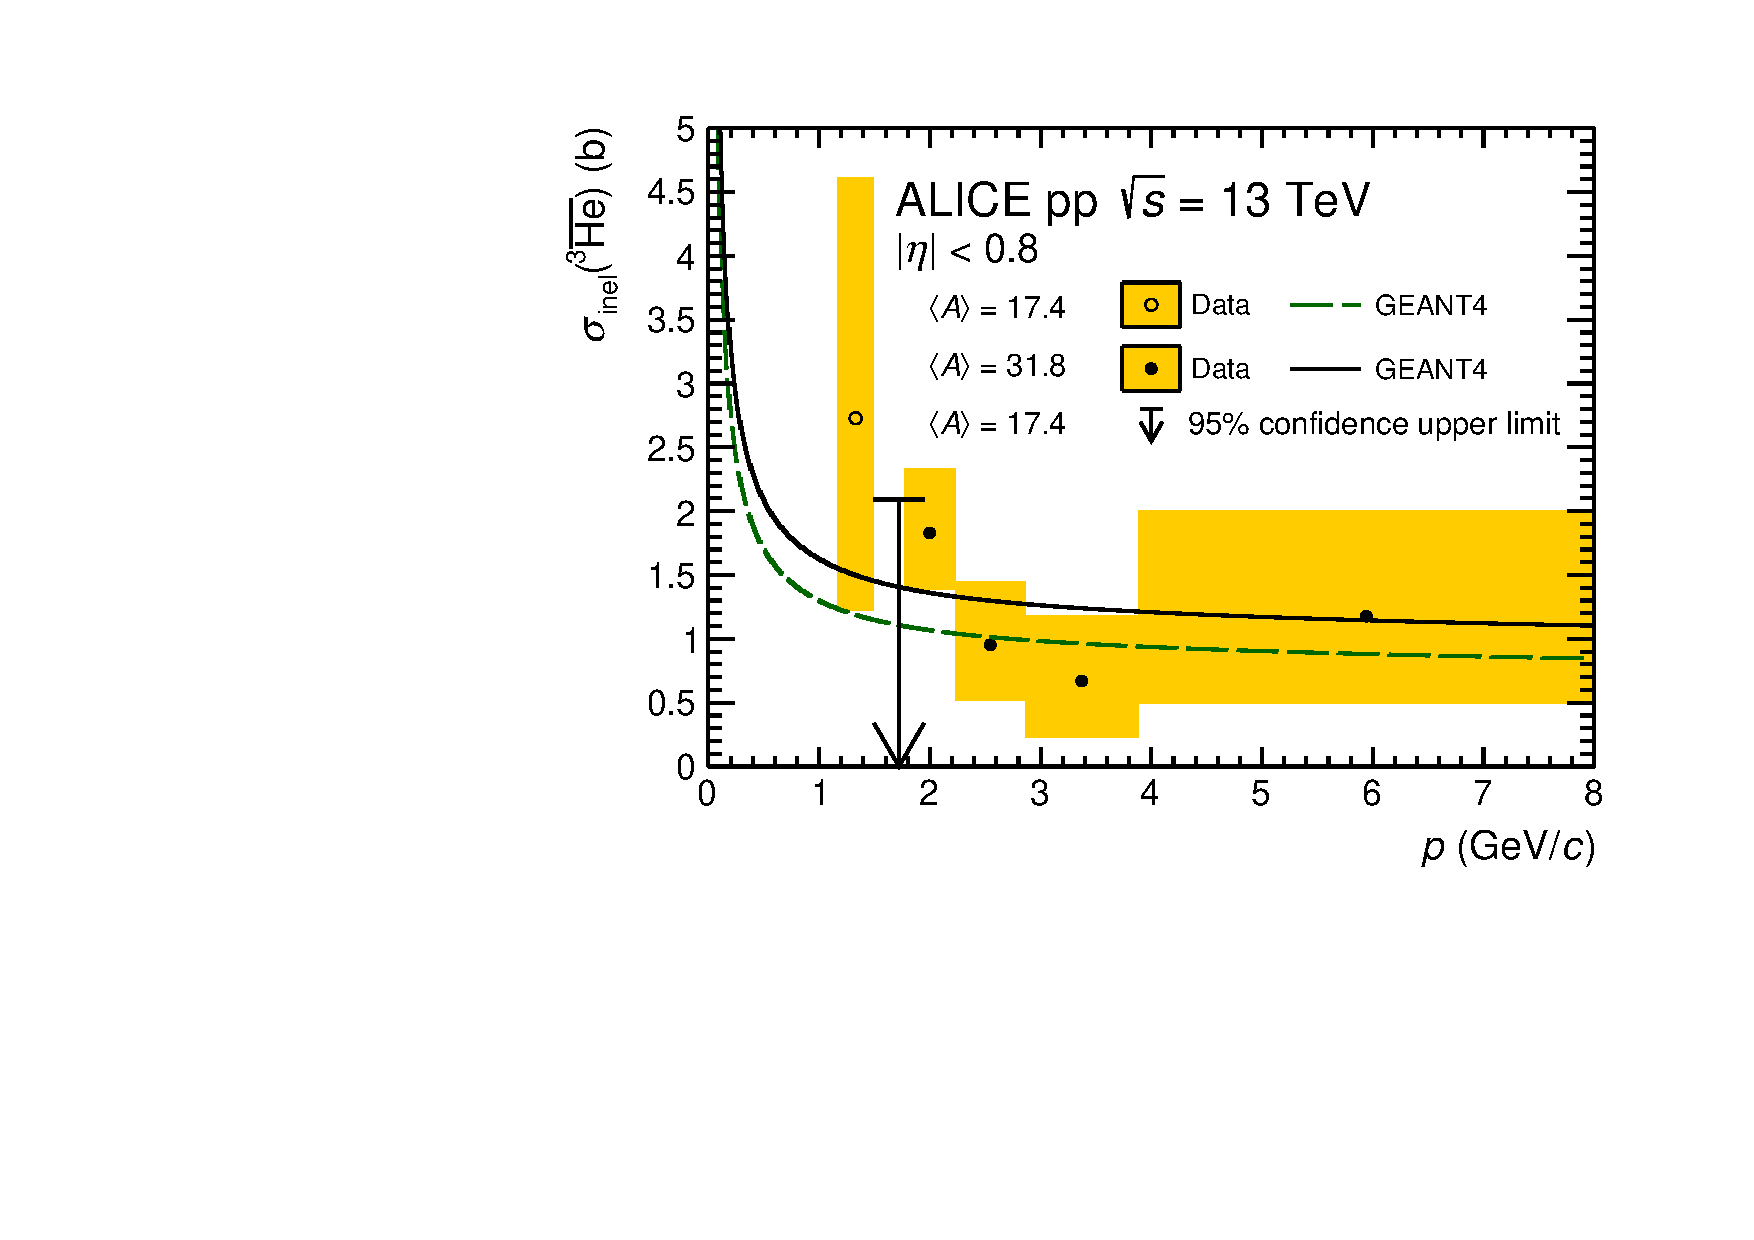
\includegraphics[width=0.48\textwidth]{figures/Antihelium_inelastic_cross_section.pdf}
    \caption{(Left) (Right) \sigmainel\ as measured using the antiparticle-to-particle method in pp collisions at $\sqrt{s}=$13 TeV. The uncertainties include both statistical and systematic uncertainties. Open points are from the analysis using the TPC only for particle identification, while closed points require a matching hit in the TOF in addition to the TPC, which therefore has a different averaged material value. The lines show the parameterization used in Geant4.}
    \label{fig:Ahe_sigma_inel_pp}
\end{figure}

The measurement of \sigmainel\ done in Pb--Pb collisions using the TOF-to-TPC method is shown for comparison in figure \ref{fig:Ahe_sigma_inel_PbPb}. The much increased statistics available for the Pb--Pb data sample results in much reduced statistical uncertainty. The two measurements are consistent with each other.

\begin{figure}
    \centering
    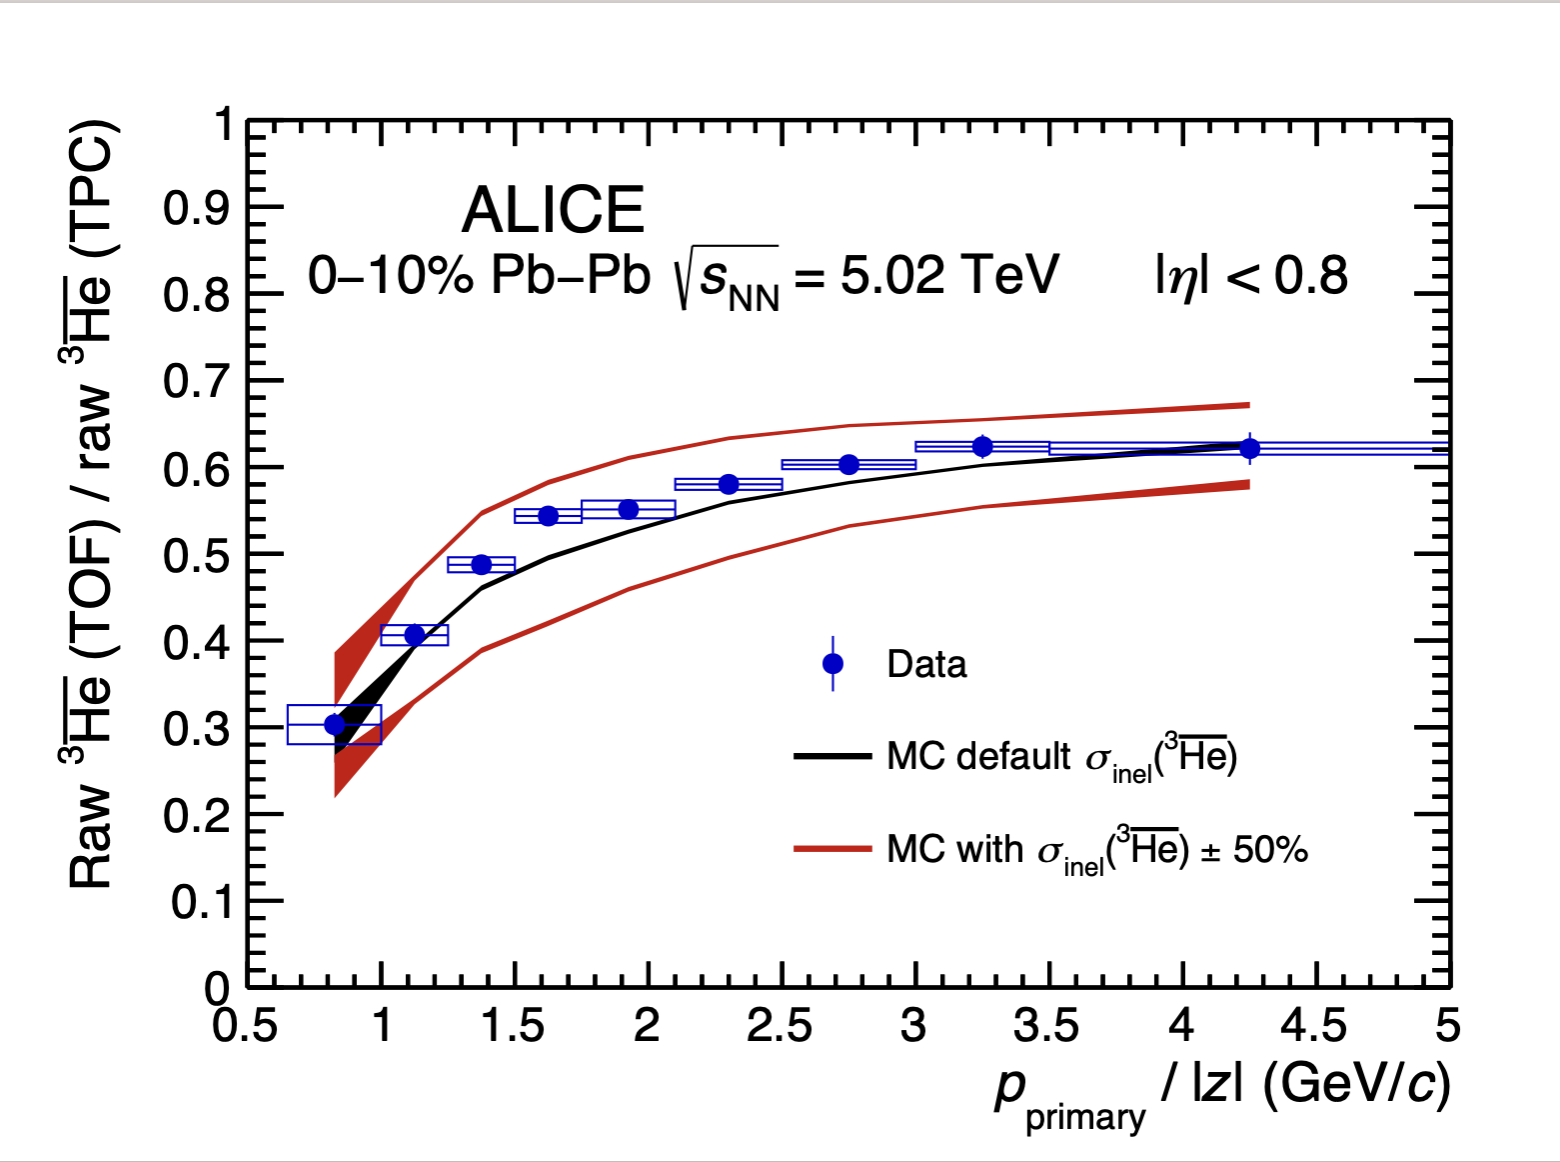
\includegraphics[width=0.48\textwidth]{figures/he3bar_TOF-to-TPC-ratio.png}
    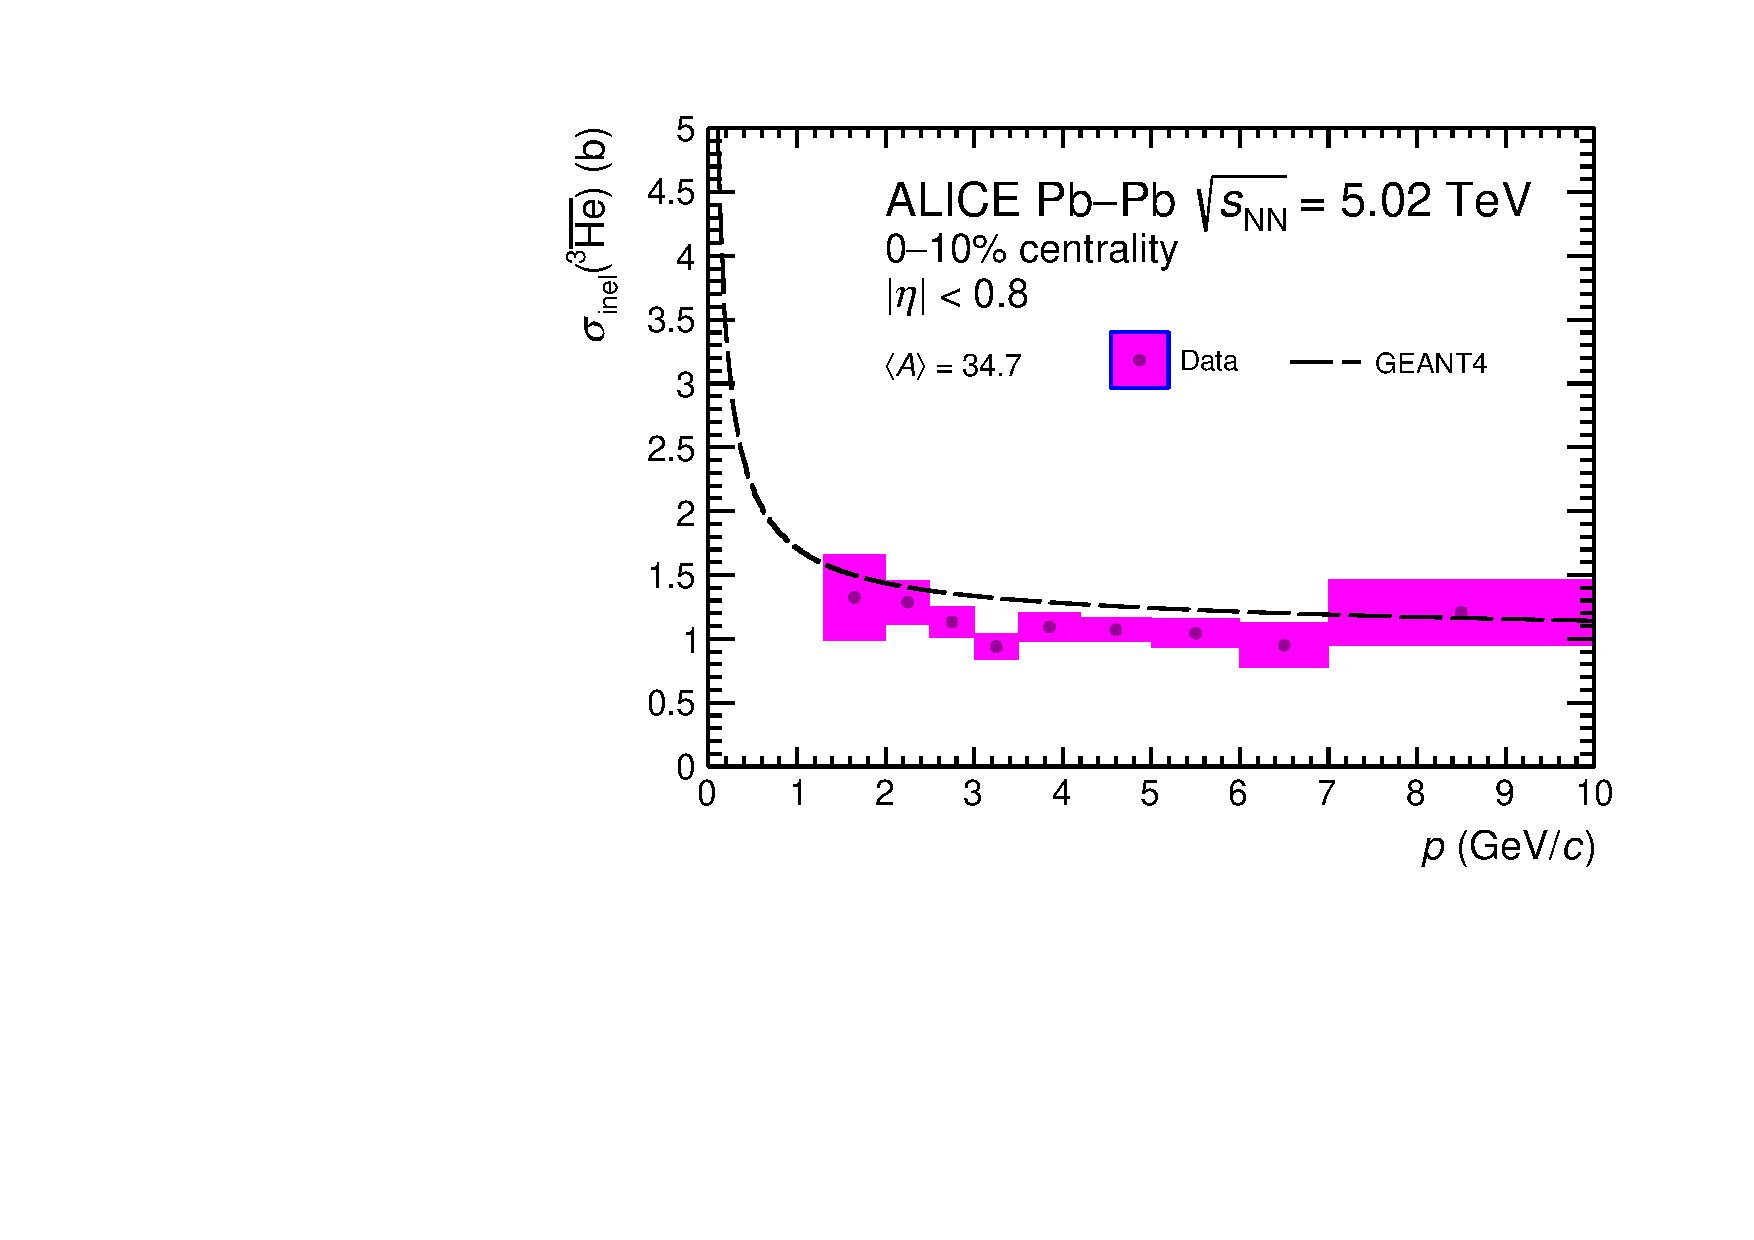
\includegraphics[width=0.48\textwidth]{figures/Antihelium_inelastic_cross_section_PbPb.pdf}
    \caption{(Left) TOF-to-TPC ratio for \ahe\ in Pb--Pb collisions at $\sqrt{s_{NN}}=$5.02 TeV. Statistical uncertainties are shown as bars, and systematic uncertainties are shown as boxes. The colored lines are the same ratio in Monte Carlo simulations with varied \sigmainel\ . (Right) \sigmainel\ as measured using the TOF-to-TPC method in Pb--Pb collisions at $\sqrt{s_{NN}}=$5.02 TeV. The uncertainties include both statistical and systematic uncertainties. The line shows the parameterization used in Geant4. Figures taken from \cite{antiHe3XS}.}
    \label{fig:Ahe_sigma_inel_PbPb}
\end{figure}

